\documentclass{article}


% if you need to pass options to natbib, use, e.g.:
%     \PassOptionsToPackage{numbers, compress}{natbib}
% before loading neurips_2023


% ready for submission
%\usepackage{neurips_2024}


% to compile a preprint version, e.g., for submission to arXiv, add add the
% [preprint] option:
\usepackage[preprint]{neurips_2024}


% to compile a camera-ready version, add the [final] option, e.g.:
%\usepackage[final]{neurips_2024}


% to avoid loading the natbib package, add option nonatbib:
%    \usepackage[nonatbib]{neurips_2023}


\usepackage[utf8]{inputenc} % allow utf-8 input
\usepackage[T1]{fontenc}    % use 8-bit T1 fonts
\usepackage{hyperref}       % hyperlinks
\usepackage{url}            % simple URL typesetting
\usepackage{booktabs}       % professional-quality tables
\usepackage{amsfonts}       % blackboard math symbols
\usepackage{nicefrac}       % compact symbols for 1/2, etc.
\usepackage{microtype}      % microtypography
\usepackage{xcolor}         % colors
\usepackage{graphicx}
\usepackage{amsmath}
\usepackage{mathtools}

\title{Uncertainty-Aware Localization Microscopy by Variational Diffusion}


% The \author macro works with any number of authors. There are two commands
% used to separate the names and addresses of multiple authors: \And and \AND.
%
% Using \And between authors leaves it to LaTeX to determine where to break the
% lines. Using \AND forces a line break at that point. So, if LaTeX puts 3 of 4
% authors names on the first line, and the last on the second line, try using
% \AND instead of \And before the third author name.


\author{%
  Clayton W. Seitz\thanks{Use footnote for providing further information
    about author (webpage, alternative address)---\emph{not} for acknowledging
    funding agencies.} \\
  Department of Physics\\
  Indiana University\\
  Indianapolis, IN 46202 \\
  \texttt{cwseitz@iu.edu} \\
  % examples of more authors
  % \And
  % Coauthor \\
  % Affiliation \\
  % Address \\
  % \texttt{email} \\
  % \AND
  % Coauthor \\
  % Affiliation \\
  % Address \\
  % \texttt{email} \\
  % \And
  % Coauthor \\
  % Affiliation \\
  % Address \\
  % \texttt{email} \\
  % \And
  % Coauthor \\
  % Affiliation \\
  % Address \\
  % \texttt{email} \\
}


\begin{document}


\maketitle


\begin{abstract}

Deep learning has recently attracted considerable attention from researchers in the natural sciences, particularly microscopists, for fast extraction of physically relevant information from images. In particular, single molecule localization microscopy (SMLM) has benefited significantly from recent advances in deep image translation. However, simple and interpretable uncertainty quantification is lacking in these applications, and remains a necessary modeling component in high-risk research. In order to quantify uncertainty in deep networks used for SMLM, we propose a generative modeling framework based on variational diffusion. This approach allows us to probe the structure of the posterior on reconstructions, creating an additional avenue toward quality control. Our model is tested on kernel density (KD) estimation in fluorescence microscopy, and we demonstrate that data augmentation with traditional SMLM architectures followed by diffusion permits simultaneous high-fidelity super-resolution with uncertainty estimation of regressed KDEs. 
\end{abstract}

\section{Introduction}

Deep learning has attracted tremendous attention from researchers in the natural sciences, with several foundational applications arising in microscopy (Weigert 2018; Falk 2019). Recently, the application of deep image translation in single-molecule localization microscopy (SMLM) has received considerable interest (Ouyang 2018; Nehme 2020; Speiser 2021). SMLM techniques are a mainstay of fluorescence microscopy and can be used to produce a pointillist representation of biomolecules in the cell at diffraction-unlimited precision (Rust 2006; Betzig 2006). In previous applications of deep models to localization microscopy, super-resolution images can be recovered from a sparse set of localizations with conditional generative adversarial networks (Ouyang 2018) or localization itself can be performed using traditional convolutional networks (Nehme 2020; Speiser 2021). Here, we focus on the latter class of models which perform KD estimation using neural networks. 

Inferences in SMLM are often made on a single measurement, and thus common measures of model performance are based on localization errors computed over ensembles of simulated images. Unfortunately, this choice precludes computation of aleatoric uncertainty at test time under a fixed model. Yet, Bayesian probability theory offers us mathematically grounded tools to reason about model uncertainty, but these usually come with a prohibitive computational cost (Gal 2022). A few approaches to avoiding this intractiblity in deep models have been mostly epistemic uncertainty quantification such as ensembling (Lakshminarayanan et al., 2017) or Monte Carlo dropout (Gal and Ghahramani, 2016). Here, we choose to model a distribution on high-resolution KDE predictions conditioned on a low-resolution input using a denoising diffusion probabilistic model (DDPM) (Ho 2020; Song 2021). Such models are one class of \emph{score based generative models} which implicitly compute the score of the data distribution at each noise scale starting from pure noise (Song 2021). 

Variational perspectives on diffusion have also been studied (Tzen 2019; Huang 2021; Vahdat 2021).  A
primary advantage of this approach is that it provides an intuitive expression of the variational lower bound in terms of the signal-to-noise ratio of the diffused data, leading to much simplified expressions of the loss. Moreover, recent efforts have shown that the variational bound can be reparameterized to give a class of conventional diffusion losses with superior performance, for example the widely used noise estimation loss (Ho 2020). 

In the remainder of this paper, we first introduce the likelihood of low-resolution images in localization microscopy, and show uncertainty quantification in a rudimentary example scenario. Then, we introduce kernel density estimation as an alternative to direct localization using low-resolution images, and conclude by demonstrating our variational diffusion model for measuring uncertainty KD estimation at scale. 

\section{Background}

\subsection{Image Likelihood and Localization Error}

The central objective of single molecule localization microscopy is to infer a set of molecular coordinates $\theta$ from measured low resolution images $\bold{x}$. The likelihood on a particular pixel $p(\bold{x}_k|\theta)$ is taken to be a convolution of Poisson and Gaussian distributions, due to shot noise $p(s_{k}) = \mathrm{Poisson}(\omega_{k})$ and sensor readout noise $p(\zeta_{k}) = \mathcal{N}(o_{k},w_{k}^{2})$ 

\begin{equation}
p(\bold{x}_{k}|\theta) = A\sum_{q=0}^{\infty} \frac{1}{q!}e^{-\omega_{k}}\omega_{k}^{q}\frac{1}{\sqrt{2\pi}\sigma_{k}}e^{-\frac{(\bold{x}_{k}-g_{k}q-o_{k})}{2\sigma_{k}^{2}}} \approx \mathrm{Poisson}(\omega_{k}')
\end{equation}


\begin{figure}
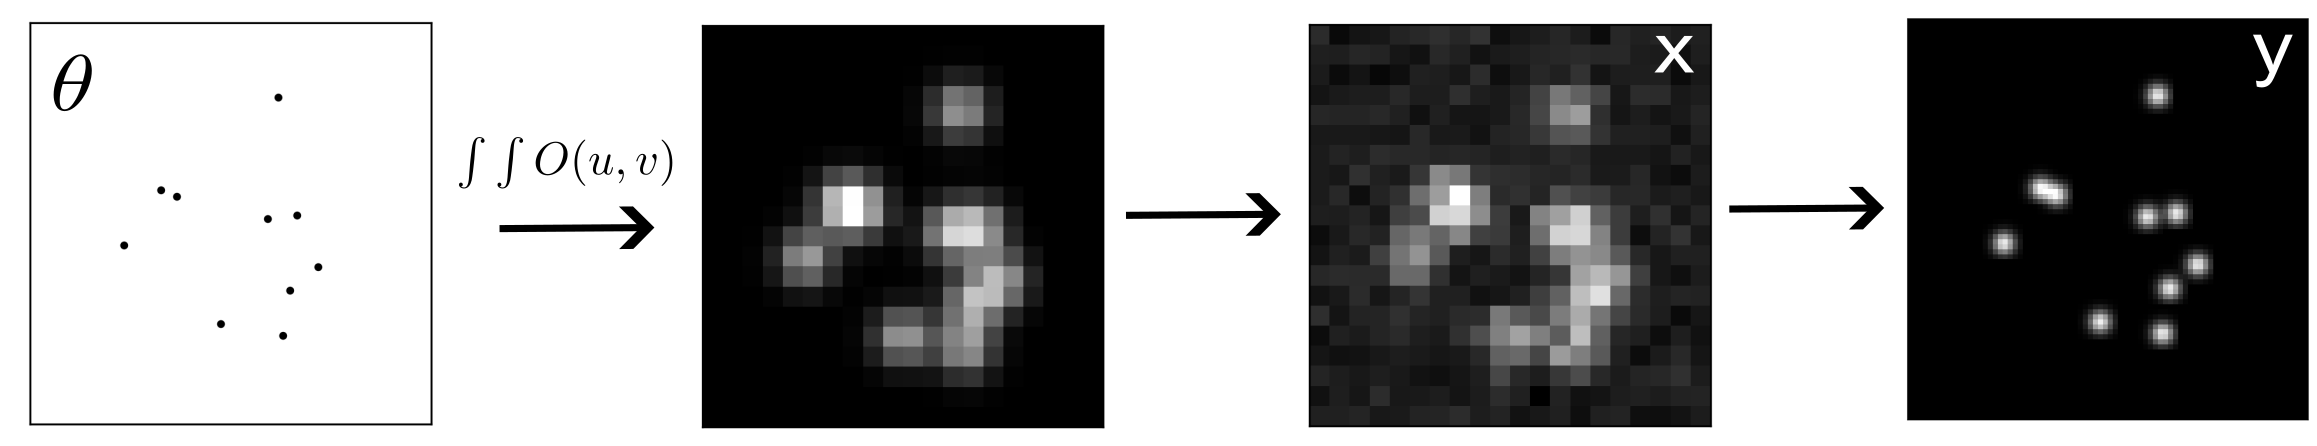
\includegraphics[scale=0.225]{Generation.png}
\caption{Generative model of single molecule localization microscopy images. Low resolution images $\bold{x}$ are generated from coordinates $\theta$ by integration of the optical transfer function $O$ and sampling from the likelihood (1): $\bold{x}\sim p(\bold{x}|\theta) = \prod_{k} p(\bold{x}_k|\theta)$. A kernel density estimate $\bold{y}$ is inferred from $\bold{x}$}
\end{figure}

where $A$ is some normalization constant. After subtraction of a known offset $o_{k}$ of the pixel array, which can be easily measured, we have $\omega_{k}' = \omega_{k} + w_{k}^{2}$. For the sake of generality, we include a per-pixel gain factor $g_{k}$, which is often unity. Sampling from $p(\bold{x}_{k}|\theta)$ is trivial; however, for computation of a lower bound on uncertainty in $\theta$, the summation in (1) can be difficult to work with. Therefore, we choose to use a Poisson approximation for simplification, valid under a range of experimental conditions (Huang 2013). The expectation of the Poisson process $\omega_{k}$ at each pixel of the image must then be computed from the optical impulse response $O(u,v)$, which is taken to be an isotropic Gaussian in two-dimensions. Consider an idealized scenario where an isolated fluorescent molecule exists in the image plane. For a particular pixel of width $\delta$ centered at $\xi_{k}=(u_k,v_k)$ in the first dimension, we define

\begin{equation}
\Delta E_{\theta_{i}} \vcentcolon = \int_{\xi_{k,i}-\delta /2}^{\xi_{k,i}+\delta /2} O(u;\theta_{i})du = \frac{1}{2}\left(\mathrm{erf}\left(\frac{\xi_{k,i}+\frac{\delta}{2}-\theta_{i}}{\sqrt{2}\sigma_{\bold{x}}}\right) -\mathrm{erf}\left(\frac{\xi_{k,i}-\frac{\delta}{2}-\theta_{i}}{\sqrt{2}\sigma_{\bold{x}}}\right)\right)
\end{equation}

The expected value at each pixel is then $\omega_{k}\propto \prod_{\theta_{i}\in \theta} \Delta E_{\theta_{i}}(\xi_{k,i},\theta_{i},\sigma_{\bold{x}}) $. Using this, sampling from (1) is can be carried out by $\bold{x}_{k} = s_{k} + \zeta_{k}$ for $s_{k}\sim \mathrm{Poisson}(\omega_{k}), \eta_{k}\sim \mathcal{N}(o_{k},w_{k}^{2})$. The complete generative process is depicted in Figure 1. 

\subsection{Gaussian kernel density estimation}

Direct optimization of the likelihood in (1) from observations $\bold{x}$ alone is challenging when fluorescent emitters are dense within the field of view and fluorescent signals significantly overlap. However, convolutional neural networks (CNN) have recently proven to be powerful tools fluorescence microscopy to extract parameters describing fluorescent emitters such as color, emitter orientation, $z$-coordinate, and background signal (Zhang 2018; Kim 2019; Zelger 2018). For localization tasks, CNNs typically employ upsampling layers to reconstruct Bernoulli probabilities of emitter occupancy (Speiser 2021) or kernel density estimates with higher resolution than experimental measurements (Nehme 2020). We choose to use kernel density estimates in our model, denoted by $\bold{y}$, which are latent in the low-resolution data $\bold{x}$. KDEs are the most common data structure used in SMLM, and can be easily generated from molecular coordinates, alongside observations $\bold{x}$, using well-understood models of the optical impulse response (Zhang 2007). 

\begin{figure}
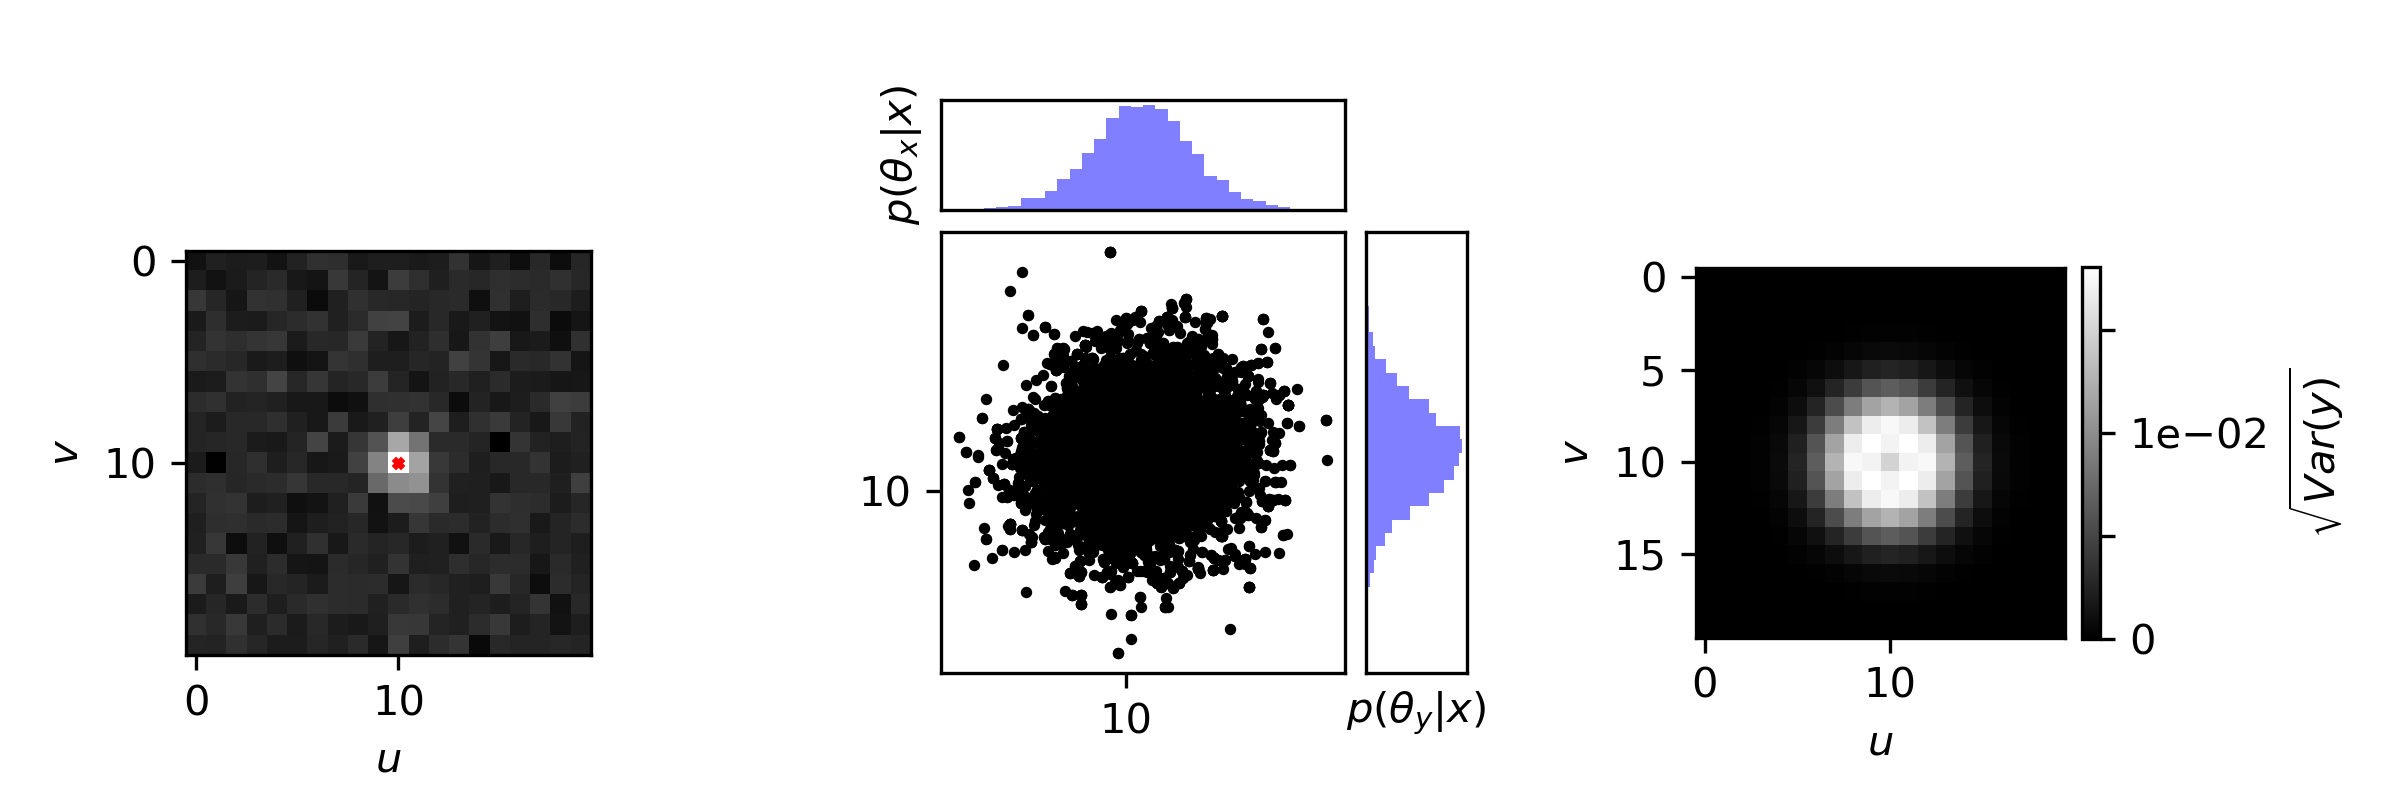
\includegraphics[scale=0.7]{MCMC.png}
\caption{Monte Carlo estimation of the marginal variances $\sqrt{\mathrm{Var}(\bold{y}_k)}$ for an isolated fluorescent emitter. MCMC sampling is carried out using the low-resolution image (left) to estimate the posterior (middle) and generate an image of marginal variances (right)}
\end{figure}

Similar to the generative process on low resolution images $\bold{x}$, we can generate KDEs $\bold{y}$ by repurposing the generative model (1) on an unsampled image without noise. In other words, we cast Gaussian kernel density estimation as a noiseless image generation process on the domain of $\bold{y}$. Under a fixed configuration of $N$ particles $\theta$, the value of an non-normalized KDE pixel $\bold{y}_{k}$ is given by

\begin{equation}
\bold{y}_{k}(\theta) = \sum_{n=1}^{N}\Delta E_{\theta_x}(u_{k},\theta_{n,x},\sigma_{\bold{y}}) \Delta E_{\theta_y}(v_{k},\theta_{n,y},\sigma_{\bold{y}})
\end{equation}

where the hyperparameter $\sigma_{\bold{y}}$ is the Gaussian kernel width. 

\section{Uncertainty-Aware Localization Microscopy by Variational Diffusion}

We consider datasets $(\bold{x}_i,\bold{y}_{0,i},\hat{\bold{y}}_{i})_{i=1}^{N}$ of observed images $\bold{x}_i$ true kernel density estimate (KDE) images $\bold{y}_{0,i}$, and augmented low-resolution inputs $\hat{\bold{y}}_{i}=\phi(\bold{x}_{i})$, where $\phi$ is a separate deep network. Observations $\bold{x}_i$ are simulated under the convolution distribution (1) and KDEs are generated by (4).

\subsection{Problem Statement}

Point estimates $\hat{\bold{y}}_{i}$ produced by the traditional deep architectures for localization microscopy produce strong results, but lack uncertainty quantification. In principle, distribution on $\bold{y}_{k}$ is given directly from $p(\theta|\bold{x})$, which can be estimated by Metropolis-Hastings MCMC (Figure 2). Unfortunately, the posterior $p(\theta|\bold{x})$ has no known analytical form and can be difficult to compute at test time, since (i) molecules cannot be easily resolved and therefore $\theta$ is of unknown dimension and (ii) $\theta$ can be high dimensional and efficient exploration of the parameter space is challenging. The central goal of this paper is to instead model a conditional distribution on the latent $\bold{y}$: $p(\bold{y}|\bold{x})$, where $\bold{y}$ is of known dimensionality. We choose to model $p(\bold{y}|\bold{x})$ with a diffusion model, given that the distribution $p(\bold{y}|\bold{x})$ is expensive to compute, even if $p(\theta|\bold{x})$ were known.

Recent advances in generative modeling, particularly diffusion models (Sohl-Dickstein 2015; Ho 2020; Song 2021) present a unique opportunity to integrate uncertainty awareness into the localization microscopy toolkit. However, sampling from diffusion models can be computationally expensive, given that generation amounts to solving a complex stochastic differential equation, effectively mapping a simple base distribution to the complex data distribution. The solution of such equations requires numerical integration with very small step sizes, resulting in thousands of neural network evaluations (Saharia 2021; Vahdat 2021). For conditional generation tasks in high-risk applications, generation complexity is further exacerbated by the need for the highest level of detail in generated samples. Moreover, in the present application, modeling the posterior is far more important than diversity in generated samples. Therefore, we propose that sampling is preceded by an augementation network $\phi$, which in essence generates an initial estimate to guide the diffusion process. Reasoning for this choice in our application is two-fold:

\textbf{Synthesis Speed}. By training the augmentation network $\phi$ to obtain an approximate estimate of $\bold{y}_{0}$, we can reduce the number of iterations, since the diffusion model only needs to model the remaining mismatch, resulting in a less complex model from which sampling becomes easier. Speed is critical in SMLM applications, which can produce thousands of images in a single experiment.\\

\textbf{Sample Fidelity}. Since Langevin dynamics will often be initialized in low-density regions of the data distribution, inaccurate score estimation in these regions will negatively affect the sampling process (Song 2019). Moreover, mixing can be difficult because of the need of traversing low density regions to transition between modes of the distribution. Preprocessing with a deterministic neural network $\phi$ can ameliorate this issue, by aiding score estimation in low density regions. 



%Here, the model $\phi$ is realized by a CNN with upsampling layers. Consider the Markov chain wherein the KDE $\bold{y}_{0}$ is latent in and inferred from a noisy measurement $\bold{x}$, i.e., $\bold{y}_{0}\rightarrow \bold{x} \xrightarrow[]{\phi}\bold{\hat{y}}$. By the data processing inequality any function $\phi$ can only destroy information in $\bold{x}$ pertaining to $\bold{y}_{0}$ i.e., $I(\bold{x};\bold{y}_0) \geq I(\bold{\hat{y}};\bold{y}_0)$ or $h(\bold{y}_0|\bold{\hat{y}}) \geq h(\bold{y}_0|\bold{x})$ where $I$ is the mutual information and $h$ is the entropy. This suggests that the uncertainty in $p_{\psi}(\bold{y}_0|\bold{\hat{y}})$ is an upper bound on the entropy of $p(\bold{y}_0|\bold{x})$. This however does not imply that the distributions should be equivalent, nor does it necessarily apply to the marginal variance of each pixel of the KDE. To address this during training, $p(\theta|\bold{x})$ can be estimated, and the and expectation $\bar{\bold{y}}(\theta)$ and marginal variance $\mathrm{Var} (\bold{y}(\theta))$ can be obtained by Monte Carlo estimation

%\begin{equation}
%\bar{\bold{y}}(\theta) = \underset{\theta\sim p(\theta|\bold{x})}{\mathbb{E}}\left[ \bold{y}(\theta)\right] \quad \mathrm{Var} (\bold{y}(\theta)) = \underset{\theta\sim p(\theta|\bold{x})}{\mathbb{E}}\left[ \bold{y}(\theta)-\bar{\bold{y}}(\theta)\right]^2
%\end{equation}

%which can be integrated into the loss function.




\subsection{Variational Diffusion}

\begin{figure}
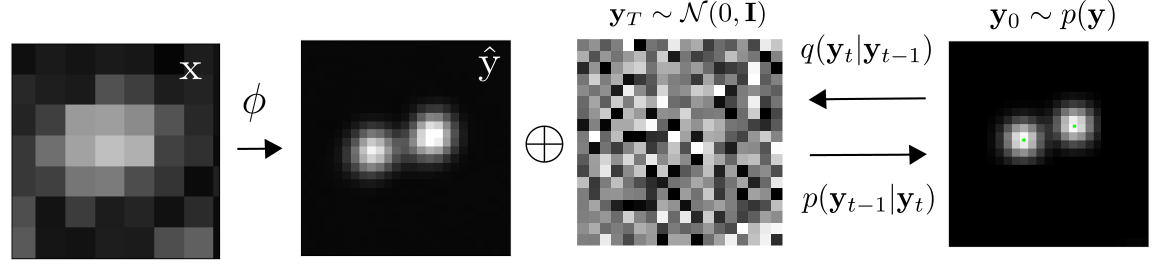
\includegraphics[scale=4.5]{Denoise.png}
\caption{Conditional diffusion model for sampling kernel density estimates. An initial KDE estimate $\bold{\hat{y}}$ is found by the CNN $\phi$, which is used as conditional input in the DDPM}
\end{figure}

Diffusion models (Sohl-Dickstein 2015; Ho 2020; Song 2021) are a class of generative models originally inspired by nonequilibrium statistical physics, which slowly destroy structure in a data distribution via a fixed Markov chain referred to as the \emph{forward process}. In the present context, we leverage a novel interpretation of this model class as likelihood-based models (Kingma 2021; Kingma 2023) to approximate the posterior $p(\bold{y}|\bold{x})$. 

\textbf{Diffusion Model}. The forward process gradually adds Gaussian noise to the latent KDE $\bold{y}_0$ according to a variance schedule $\beta_{0:T}$

\begin{equation}
q(\bold{y}_{T}|\bold{y}_{0}) = \prod_{t=1}^{T}q(\bold{y}_{t}|\bold{y}_{t-1}) \;\;\; q(\bold{y}_{t}|\bold{y}_{t-1}) = \mathcal{N}\left(\sqrt{1-\beta_{t}}\bold{y}_{t-1},\beta_t I\right)
\end{equation}

The usual procedure is then to learn a parametric representation of the \emph{reverse process}, and therefore generate samples from  $p(\bold{y}_{0}|\bold{\hat{y}})$, starting from noise. Formally, $p_{\psi}(\bold{y}_{0}|\bold{\hat{y}}) = \int p_{\psi}(\bold{y}_{0:T}|\bold{\hat{y}})d\bold{\hat{y}}_{1:T}$ where $\bold{y}_{t}$ is a latent representation with the same dimensionality of the data and $p_{\psi}(\bold{y}_{0:T}|\bold{\hat{y}})$ is a Markov process, starting from a noise sample $p_{\psi}(\bold{y}_{T}) = \mathcal{N}(0,I)$. 

\begin{equation}
p_{\psi}(\bold{y}_{0:T}) = p_{\psi}(\bold{y}_{T})\prod_{t=1}^{T} p_{\psi}(\bold{y}_{t-1}|\bold{y}_{t}) \;\;\; p_{\psi}(\bold{y}_{t-1}|\bold{y}_{t}) = \mathcal{N}\left(\mu_{\psi}(\bold{y}_{t}),\beta_{t}I\right)
\end{equation}

where we reuse the variance schedule of the forward process (Ho 2020). From (7) it can be seen that the learnable parameter in the reverse process is the expectation of the transition $\mu_{\psi}$ where $\psi$ is a neural network. We omit conditioning on $\hat{\bold{y}}$ for each transition density $p_{\psi}(\bold{y}_{t-1}|\bold{y}_{t})$, as this is only considered at the first step of the reverse process i.e., $p_{\psi}(\bold{y}_{T-1}|\bold{y}_{T},\hat{\bold{y}})$. An important property of the forward process is that it admits sampling $\bold{y}_t$ at an arbitrary timestep $t$ in closed form (Ho 2020). Using the notation $\alpha_t := 1 - \beta_t$ and $\gamma_t := \prod_{s=1}^{t} \alpha_s$, we have $q(\bold{y}_t|\bold{y}_0) = \mathcal{N} \left(\sqrt{\gamma_{t}} \bold{y}_{0}, (1 - \gamma_t)I \right)$ or $\bold{y}_{t} = \sqrt{\gamma_{t}}\bold{y}_{0} + \sqrt{1-\gamma_{t}}\bold{\epsilon}$ for $\epsilon \sim \mathcal{N}(0,I)$. Learning the reverse process can be approached by either regressing the starting noise $\bold{\epsilon}$ or the true KDE $\bold{y}_{0}$ as there is a deterministic relationship between the two given by the forward process. We adopt the former for consistency with other work, and define $s_{\psi}$ as a neural denoising function which regresses the noise $\bold{\epsilon}$ from $\bold{\hat{y}}$. Importantly, the noise estimate $\epsilon_{\psi}$ and $\mu_{\psi}$ are related by (Saharia 2021)

\begin{equation}
\mu_{\psi}(\bold{y}_{t},\gamma_{t}) = \frac{1}{\sqrt{1-\beta_{t}}}\left(\bold{y}_{t} - \frac{\beta_{t}}{\sqrt{1-\gamma_{t}}}\epsilon_{\psi}\right)
\end{equation}

which forms the basic mechanism for transitions in the reverse process: $\bold{y}_{t-1} = \mu_{\psi}(\bold{y}_{t},\gamma_{t}) + \sqrt{\beta_{t}}\xi_{t}$, for $\xi_{t} = \mathcal{N}(0,I)$.

\textbf{Variational Objective}. Following (Kingma 2021), we define our generative model by inverting a diffusion process, yielding a hierarchical generative model that samples a sequence of latents $\bold{y}_{t}$, with time running backward. Training of the model is achieved through the usual variational bound

\begin{equation}
-\log p(\bold{x}) \leq -\mathbb{E}_{q(\bold{y}_{0}|\bold{x})} \log p(\bold{x}|\bold{y}_{0}) + D_{KL}(q(\bold{y}_{T}|\bold{x}) || p(\bold{y}_{T})) + \mathcal{L}_{\psi} = \mathrm{VLB}(\bold{x})
\end{equation}

We focus on the diffusion loss $\mathcal{L}_{\psi}$, which is the only relevant term in the above objective (Rebeira 2024)

\begin{equation}
\mathcal{L}_{\psi} = \sum_{i=1}^{T} \mathbb{E}_{q_{\psi}(\bold{y}_{t}|\bold{x})} [ D_{KL}(q_{\psi}(\bold{y}_{t-1}|\bold{y}_{t},\bold{x}) || p(\bold{y}_{t-1}|\bold{y}_{t},\bold{x})) ]
\end{equation}

In a diffusion model $p(\bold{y}_{t-1}|\bold{y}_{t},\bold{x}) = q(\bold{y}_{t-1}|\bold{y}_{t},\hat{\bold{x}}_{\psi})$ which is modeled by $p_{\psi}(\bold{y}_{t-1}|\bold{y}_{t}) = \mathcal{N}\left(\mu_{\psi}(\bold{y}_{t}),\beta_{t}I\right)$. Importantly, $D_{KL}(q_{\psi}(\bold{y}_{t-1}|\bold{y}_{t},\bold{x}) || p(\bold{y}_{t-1}|\bold{y}_{t},\bold{x}))$ and therefore, the variational bound, are closely linked to the common noise estimation loss used in DDPMs (Ho 2020; Kingma 2021). 

We use the following Monte Carlo estimate of $\mathcal{L}_{\psi}$, which demonstrates that the variational bound can be written in terms of the common noise-estimation loss

\begin{equation}
\mathcal{L}_{\psi} = \frac{T}{2}\mathbb{E}_{\epsilon\sim \mathcal{N}(0,I),t\sim U(1,T)}[\left(\frac{\mathrm{SNR}(t-1)}{\mathrm{SNR}(t)}-1\right)\lvert\lvert \bold{\epsilon}-\bold{\epsilon}_{\psi}(\bold{y}_{t})\lvert\lvert_{2}^{2}]
\end{equation}

where $\mathrm{SNR}(t) = \gamma_{t}/\beta_{t}$. Full details of this derivation can be found in (Kingma 2021; Rebeira 2024) and are outlined in Appendix A. 


\section{Experiments}

All training data consits of low-resolution $20\times 20$ images, setting $\sigma_{\bold{x}}=0.92$ in units of low-resolution pixels, for consistency with common experimental conditions with a 60X magnification objective lens and numerical aperture (NA) of 1.4. We choose $i_{0}=200$ for experiments for consistency with typical bright fluorophore emission rates. All KDEs have dimension $80\times 80$, are scaled between $[0,1]$, and are generated using $\sigma_{\bold{y}}=3.0$ pixels in the upsampled image. For a typical CMOS camera, this results in KDE pixels with lateral dimension of $\approx 27\mathrm{nm}$. Initial coordinates $\theta$ were drawn uniformly over a two-dimensional disc with a radius of 7 low-resolution pixels.

\begin{figure}
\centering
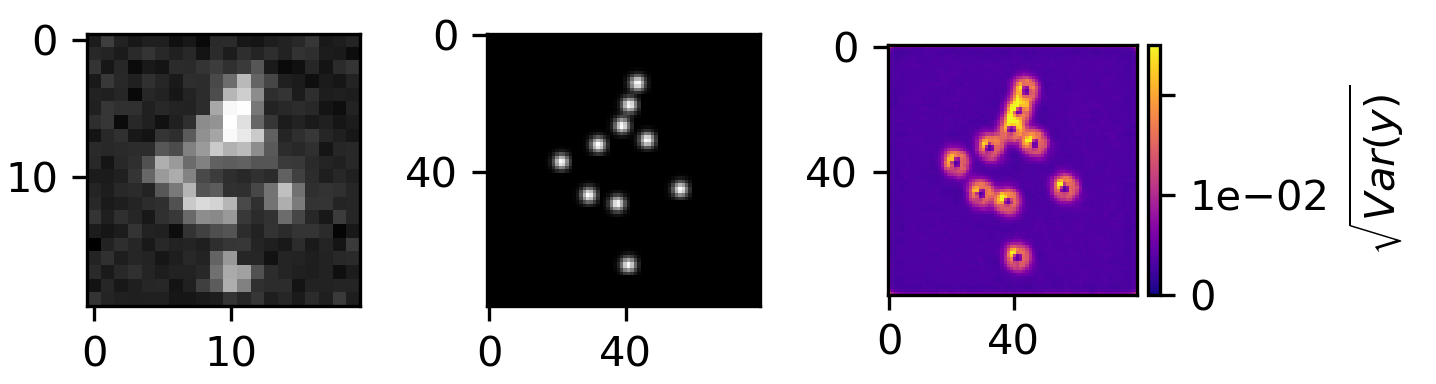
\includegraphics[scale=1.1]{Bayes.png}
\caption{Non cherry-picked estimation of marginal variances. A low-resolution image $\bold{x}$ (left column) is transformed by $\phi$ to produce a KDE estimate $\hat{\bold{y}}$ (middle column) and a DDPM $\psi$ computes a map of marginal variances (right column)}
\end{figure}

\textbf{Localization RMSE}. In order to verify the initial predictions made by the augmentation model $\phi$, we simulated a dataset $(\bold{x}_i,\bold{y}_{0,i},\hat{\bold{y}}_{i})_{i=1}^{N}$ with $N=1000$, and  detect objects in the predicted $\hat{\bold{y}}_{i}$ using the Laplacian of Gaussian (LoG) detection algorithm (Lindeberg 2013). Localization is carried out from scale-space maxima directly in LoG, as opposed to fitting a model function to KDE predictions. A particular LoG localization in the KDE is paired to the nearest ground truth localization and is unpaired if a localization is not within 5 KDE pixels of any ground truth localization. In addition to localization error, we measure a precision $\mathrm{P = TP/(TP + FP)} = 1.0$ and recall $\mathrm{R = TP/(TP + FN)} = 0.85$, where $\mathrm{TP}$ denotes true positive localizations, $\mathrm{FP}$ denotes false positive localizations, and $\mathrm{FN}$ denotes false negative localizations.


\textbf{Variational Diffusion}. We set $T = 100$ for all experiments and treat forward process variances $\beta_{t}$ as hyperparameters, with a linear schedule from $\beta_{0}=10^{-4}$ to $\beta_{T}=10^{-2}$.
These constants were chosen to be small relative to ground truth KDEs, which are scaled to $[-1,1]$, ensuring that forward process distribution $\bold{y}_{T}\sim q(\bold{y}_{T}|\bold{y}_{0})$ approximately matches the reverse process $\bold{y}_T\sim \mathcal{N}(0, I)$ at $t=T$.


\section{Conclusion}

We proposed a variational diffusion model for uncertainty-aware localization microscopy. Our approach builds on recent advancements in conditional diffusion models, to model the posterior distribution on high-resolution kernel density estimates (KDE) from low-resolution inputs. This tractable posterior distribution is constructed by first augmenting low resolution inputs to a KDE estimate using a modified form of the DeepSTORM architecture (Nehme 2020). Conditioning a DDPM on this initial estimate permits sampling with relatively fewer samples than most existing DDPMs in similar applications, thereby making computation of marginal variances possible. Our approach made three core contributions: (i) we derived a relationship between the posterior on kernel density estimates with the posterior on molecular locations, and (ii) we demonstrated that a diffusion model can model a distribution on KDEs with qualitatively similar marginal variances expected from predictions made using MCMC. By using a recently discovered relationship of the variational lower bound to a traditional noise-estimation objective, we can confidently approximate the true posterior.

\section{Broader Impact}

The development of a method for uncertainty estimation in super-resolution imaging, as proposed here, holds profound implications beyond its immediate application in single-molecule localization microscopy (SMLM). By leveraging denoising diffusion probabilistic models (DDPMs) for uncertainty estimation, this approach not only enhances the reliability of super-resolution image reconstructions but also extends its utility to a diverse array of domains. The incorporation of a guided diffusion process facilitates efficient reconstruction while maintaining intepretation of the underlying uncertainty. Importantly, the principles underlying this method resonate across various fields, suggesting its potential applicability in domains beyond microscopy. For instance, the extension of similar techniques to general image resolution highlights the potential to address uncertainty in a wide range of bioimaging or medical imaging tasks. Moreover, the utilization of diffusion models for uncertainty estimation aligns with a broader trend in leveraging probabilistic frameworks for enhancing deep learning applications, with implications extending to fields such as natural language processing, computer vision, and autonomous systems. By bridging these interdisciplinary boundaries, this method not only addresses a critical need in localization microscopy but also contributes to the advancement of uncertainty-aware deep learning methodologies with far-reaching societal impacts. From improving medical diagnostics to enhancing environmental monitoring, the implications of this work reverberate across diverse applications, underscoring its potential to drive innovation and progress in numerous fields.

\section*{References}


{
\small


[1] Nehme, E., et al. DeepSTORM3D: dense 3D localization microscopy and PSF design by deep learning. Nature Methods 17, 734–740 (2020).


[2] Ouyang, W., et al. Deep learning massively accelerates super-resolution localization microscopy. Nature Biotechnology 36, 460–468 (2018).


[3] Speiser, A., et al. Deep learning enables fast and dense single-molecule localization with high accuracy. Nature Methods 18, 1082–1090 (2021).

[4] Sohl-Dickstein J., et al. Deep unsupervised learning using nonequilibrium thermodynamics. ICLR (2015).

[5] Ho J., et al. Denoising Diffusion Probabilistic Models. Advances in Neural Information Processing Systems (2015).

[6] Nanxin C., et al. WaveGrad: Estimating Gradients for Waveform Generation
. ICLR (2021).

[7] Chao, J., et al. Fisher information theory for parameter estimation in single molecule microscopy: tutorial. Journal of the Optical Society of America A 33, B36 (2016). 

[8] Schermelleh, L. et al. Super-resolution microscopy demystified. Nature Cell Biology vol. 21 72–84 (2019). 

[9] Zhang, B., et al. Gaussian approximations of fluorescence microscope point-spread function models. (2007). 

[10] Smith, C.S.,  Fast, single-molecule localization that achieves theoretically minimum uncertainty. Nature Methods 7, 373–375 (2010). 

[11] Nieuwenhuizen, R., et al. Measuring image resolution in optical nanoscopy. Nature Methods 10. 557-562 (2013). 

[12] Huang, F., et al. Video-rate nanoscopy using sCMOS camera-specific single-molecule localization algorithms. Nat Methods 10, 653–658 (2013). 

[13] Rust, M., et al. Sub-diffraction-limit imaging by stochastic optical reconstruction microscopy (STORM). Nat Methods 3, 793–796 (2006).

[14] Betzig, E., et al. Imaging intracellular fluorescent proteins at nanometer resolution. Science 313, 1642–1645 (2006).

[15] Weigert, M., et al. Content-aware image restoration: pushing the limits of fluorescence microscopy. Nat. Methods 15, 1090 (2018).

[16] Falk, T., et al. U-net: deep learning for cell counting, detection, and morphometry. Nat. Methods 16, 67–70 (2019).

[17] Boyd, N., et al. DeepLoco: fast 3D localization microscopy using neural networks. Preprint at bioRxiv https://doi.org/10.1101/267096 (2018)

[18] Zelger, P., et al. Three-dimensional localization microscopy using deep learning. Opt. Express 26, 33166–33179 (2018)

[19] Zhang, P., et al. Analyzing complex single-molecule emission patterns with deep learning. Nat. Methods 15, 913 (2018)

[20] Song, Y., et al. Score-based generative model through stochastic differential equations. ICLR (2021). 

[21] Vahdat, A., et al. Score-based generative modeling in latent space. NeurIPS (2021). 

[22] Kingma, D., et al. Auto encoding variational bayes. Preprint at arXiv 
https://doi.org/10.48550/arXiv.1312.6114 (2013). 

[23] Song, Y., et al. Generative modeling by estimating gradients of the data distribution. NeurIPS (2019). 

[24] Kong, X., et al. Information theoretic diffusion. ICLR (2023). 

[25] Kong, L., et al. SDE-Net: Equipping Deep Neural Networks with Uncertainty Estimates. ICML (2020). 

[26] van Amersfoort, J., et al. Uncertainty Estimation Using a Single Deep Deterministic Neural Network. Preprint at arXiv https://doi.org/10.48550/arXiv.2003.02037. 

[27] Zhe Liu, J., et al. Simple and Principled Uncertainty Estimation with
Deterministic Deep Learning via Distance Awareness. NeurIPS 2021. 

[28] Gal Y., et al. Bayesian uncertainty quantification
for machine-learned models in physics. Nature Physics 2022. 

[29] Gal Y., et al. Dropout as a Bayesian Approximation:
Representing Model Uncertainty in Deep Learning. ICML 2016. 

[30] Welling M., et al. Bayesian Learning via Stochastic Gradient Langevin Dynamics. ICML 2011. 

[31] Saharia, C., et al. Image Super-Resolution via Iterative Refinement. Preprint at arXiv https://doi.org/10.48550/arXiv.2104.07636 (2021)

[32] Kim, T., et al. Information-rich localization microscopy through machine learning. Nat Commun 10, 1996 (2019). 

[33] Nichol, A., et al. Improved denoising diffusion probabilistic models. Preprint at arXiv https://doi.org/10.48550/arXiv.2102.09672 (2021). 

[34] Kingma, D., et al. Understanding Diffusion Objectives as the ELBO
with Simple Data Augmentation. NeurIPS (2023). 

[35] Kingma, D., et al. Variational Diffusion Models. NeurIPS (2021). 

[35] Ribeiro, F., et al. Demystifying Variational Diffusion Models.  Preprint at arXiv https://doi.org/10.48550/arXiv.2401.06281 (2024). 

}

\appendix

\section{Appendix}

\subsection{Optical impulse response}

It is common to describe the optical impulse response of a microscope as a two-dimensional isotropic Gaussian (Zhang 2007). This is an approximation to the more rigorous diffraction models given by Richards and Wolf (1959) or Gibson and Lanni (1989). Over a continuous domain, the impulse response reads

\begin{equation*}
O(u,v) = \frac{1}{2\pi\sigma_{\bold{x}}^{2}}e^{-\frac{(u-\theta_{u})^{2}+(v-\theta_{v})^{2}}{2\sigma_{\bold{x}}^{2}}}
\end{equation*}

The above expression can be interpreted as a probability distribution over locations where a photon can be detected. Therefore, for discrete detectors, we discretize this expression by integrating over pixels. The number of photon arrivals will follow Poisson statistics, with expected value

\begin{equation*}
\omega_{k} = i_{0}\left(\int_{u_{k}-\delta /2}^{u_{k}+\delta /2} O(u; \theta_{u})du \right)\left(\int_{v_{k}-\delta /2}^{v_{k}+\delta /2} O(v;\theta_{v})dv \right)
\end{equation*}

The scalar quantity $i_{0}$ represents the amplitude of the signal, which is proportional the quantum efficiency of a pixel $\eta$, the duration of exposure, $\Delta$, and the number of photons emitter by a fluorescent molecule $N_{0}$. With no loss of generality, $\Delta = \eta = 1$ and there is a single free parameter $N_{0}$. A simple change of variables $u' = u - \theta_{u}$ and $v' = v-\theta_{v}$ gives

\begin{align*}
\omega_{k} = i_{0}\left(\int_{u_{k}-\delta /2 - \theta_{u}}^{u_{k}+\delta /2 - \theta_{u}} O(u)du \right)\left(\int_{v_{k}-\delta /2 - \theta_{v}}^{v_{k}+\delta /2 - \theta_{v}} O(v)dv \right)
\end{align*}

One of these terms can be written as 

\begin{align*}
\int_{u_{k}-\delta /2 - \theta_{u}}^{u_{k}+\delta /2 - \theta_{u}} O(u)du &= \int_{0}^{u_{k}+\delta /2 - \theta_{u}} O(u)du - \int_{0}^{u_{k}-\delta /2 - \theta_{u}} O(u)du\\
&= \frac{1}{2}\left(\mathrm{erf}\left(\frac{u_{k}+\frac{\delta}{2}-\theta_{i}}{\sqrt{2}\sigma_{\bold{x}}}\right) -\mathrm{erf}\left(\frac{u_{k}-\frac{\delta}{2}-\theta_{i}}{\sqrt{2}\sigma_{\bold{x}}}\right)\right)
\end{align*}

where we have used the common definition $\mathrm{erf}(z) = \frac{2}{\sqrt{\pi}}\int_{0}^{z}e^{-t^{2}}dt$. To simplify the notation in the main text, we define a general expression

\begin{equation*}
\Delta E_{\theta_{i}}(\xi_{k,i},\theta_{x},\sigma_{\bold{x}}) \vcentcolon = \int_{u_{k}-\delta /2}^{u_{k}+\delta /2} O(u;\theta_{i})du = \frac{1}{2}\left(\mathrm{erf}\left(\frac{\xi_{k,i}+\frac{\delta}{2}-\theta_{i}}{\sqrt{2}\sigma_{\bold{x}}}\right) -\mathrm{erf}\left(\frac{\xi_{k,i}-\frac{\delta}{2}-\theta_{i}}{\sqrt{2}\sigma_{\bold{x}}}\right)\right)
\end{equation*}

\subsection{Metropolis-Hastings MCMC}

To obtain numerical estimates of $p(\theta|\bold{x}\propto p(\bold{x}|\theta)p(\theta)$ and therefore $p(\bold{y}|\bold{x})$, for an isolated fluorescent molecule as shown in (Figure 2), we used Metropolis-Hastings Markov Chain Monte Carlo (MCMC) to estimate the posterior on coordinates. Under the Poisson approximation in (1), the model negative log-likelihood is

\begin{equation}
\ell(\bold{x}|\theta) = -\log \prod_{k} \frac{e^{-\left(\omega_{k}'\right)}\left(\omega_{k}'\right)^{n_{k}}}{n_{k}!} = \sum_{k}  \log n_{k}! + \omega_{k}' - n_{k}\log\left(\omega_{k}'\right)
\end{equation}

where $n_{k}$ is the observed number events at a pixel. MCMC is asymptotically exact, which is not guaranteed by variational methods which may rely on a Laplace approximation around the MLE. We choose a uniform prior $p(\theta)$, and Metropolis-Hastings is run for $10^4$ iterations, the first $10^{3}$ iterations are discarded as burn-in. A proposal $\theta' = \theta + \Delta\theta$ was generated with $\Delta\theta \sim \mathcal{N}(0,\sigma^{2}I)$ where $\sigma^{2}=0.05$. The acceptance probability is

\begin{equation*}
\alpha = e^{\beta(\ell(\theta)-\ell(\theta'))}
\end{equation*}

We choose $\beta=0.2$ to achieve a target acceptance rate of $0.5$.

\subsection{Cramer-Rao Lower Bound}

Reliable inference of $\theta$ from $\bold{x}$ in general requires performance metrics for model selection. We use the Fisher information as an information theoretic criteria to assess the quality of the data augmentation model $\phi$ tested here, with respect to the root mean squared error (RMSE) of our predictions of $\theta$ (Chao 2016). The Poisson log-likelihood $\ell(\bold{x}|\theta)$ is also convenient for computing the Fisher information matrix (Smith 2010) and thus the Cramer-Rao lower bound, which bounds the variance of a statistical estimator of $\theta$, from below i.e., $\mathrm{var}(\hat{\theta}) \geq I^{-1}(\theta)$. The Fisher information is straightforward to compute under the Poisson log-likelihood in (1). In general, the Fisher information is given by the expression

\begin{equation}
I_{ij}(\theta) = \underset{\theta}{\mathbb{E}}\left(\frac{\partial \ell}{\partial\theta_{i}}\frac{\partial\ell}{\partial\theta_{j}}\right) 
\end{equation}

For an arbitrary parameter, such the $\theta_{x}$ or $\theta_{y}$ coordinate, we find that, for a Poisson log-likelihood $\ell$

\begin{align*}
\frac{\partial \ell}{\partial \theta_{i}} &= \frac{\partial}{\partial \theta_{i}} \sum_{k}  \log n_{k}! + \omega_{k}' - n_{k}\log\left(\omega_{k}'\right)\\
&= \sum_{k} \frac{\partial \omega_{k}'}{\partial\theta_{i}} \left(\frac{\omega_{k}'-n_{k}}{\omega_{k}'}\right)
\end{align*}

Using this result, we can compute the Fisher information matrix $I(\theta)$

\begin{equation*}
I_{ij}(\theta) = \underset{\theta}{\mathbb{E}}\left(\sum_{k}\frac{\partial \omega_{k}'}{\partial\theta_{i}}\frac{\partial \omega_{k}'}{\partial\theta_{j}} \left(\frac{\omega_{k}'-n_{k}}{\omega_{k}'}\right)^{2}\right) = \sum_{k}\frac{1}{\omega_{k}'}\frac{\partial \omega_{k}'}{\partial\theta_{i}}\frac{\partial \omega_{k}'}{\partial\theta_{j}}
\end{equation*}

A fundamental lower bound on the variance in our estimates of $\theta$ then is found from its inverse: $\mathrm{CRLB} = I^{-1}(\theta)$. This result is used to show in (Figure 5), that the data augmentation model $\phi$ efficiently estimates molecular coordinates under the experimental conditions tested here. 

\begin{figure}
\centering
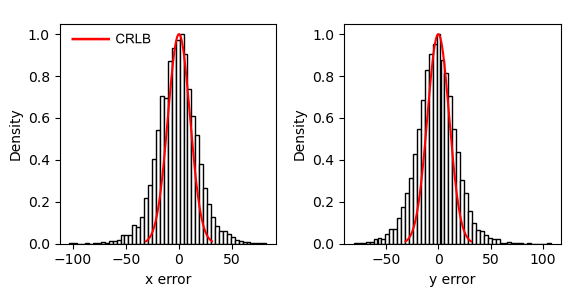
\includegraphics[scale=0.7]{Errors.png}
\caption{Localization errors of the trained model $\phi$. The Cramer-Rao lower bound is shown in red, computing by taking the diagonal elements of $I^{-1}(\theta)$.}
\end{figure}


\subsection{Neural Networks $\psi,\phi$}

\textbf{DeepSTORM CNN $\phi$}. The DeepSTORM CNN, for 3D localization, can be viewed as a deep kernel density estimator, reconstructing kernel density estimates $\bold{y}$ from low-resolution inputs $\bold{x}$. We utilize a simplified form of the original architecture for 2D localization, which we denote $\phi$ in this paper, which consists of three main modules: a multi-scale context aggregation module, an upsampling module, and a prediction module. For context aggregation, the architecture utilizes dilated convolutions to increase the receptive field of each layer. The upsampling module is then composed of two consecutive 2x resize-convolutions, computed by nearest-neighbor interpolation, to increase the lateral resolution by a factor of 4. Additional details regarding this architecture can be found in the original paper (Nehme 2020). The terminal prediction module contains three additional convolutional blocks for refinement of the upsampled image, followed by an element-wise HardTanh. The architecture is trained using the objective $\mathcal{L}_{\phi} = \frac{1}{N}\sum_{n=1}^{N} (\bold{y}_{0,n}-\bold{\hat{y}}_{n})^{2}$. 

\textbf{DDPM $\psi$}. To represent the reverse process, we used a DDPM architecture originally proposed in (Saharia 2021) where the full model is described. We chose a U-Net backbone to have channel multipliers $[1,2,4,8,8]$ in the downsampling and upsampling paths of the architecture. Parameters are shared across time, which is specified to the network using the Transformer sinusoidal position embedding. We use self-attention at the $16 \times 16$ feature map resolution. To condition the model on the input $\bold{\hat{y}}$, we concatenate the $\bold{\hat{y}}$ estimated by DeepSTORM along the channel dimension, which are scaled to $[0,1]$, with $\bold{y}_T\sim \mathcal{N}(0, I)$. Others have experimented with more sophisticated methods of conditioning, but found that the simple concatenation yielded similar generation quality (Saharia 2021). 

\end{document}
